\chapter{Introduction: The New Era of IT Consulting}

\section{The Changing Landscape}

The IT consulting world is undergoing a seismic shift. According to Deloitte's recent report, ``Unleashing value from digital transformation: Paths and pitfalls,'' the days of strategy-only consulting are numbered. Clients now demand execution, and technology is at the heart of it all.

\begin{importantbox}
Consider this: 30 years ago, classic strategy work made up 60-70\% of consulting engagements. Today? It's down to a mere 20\%. The message is clear: consultants who can't deliver tangible, tech-driven results will be left behind.
\end{importantbox}

However, this shift presents an exciting opportunity for small firms. With the right tools and knowledge, you can deliver outcomes that rival the big players, at a fraction of the cost.


\section{The Power of Automation}

Automation is not just a buzzword; it's your ticket to:

\begin{itemize}
    \item Boosting productivity by eliminating time-consuming manual tasks
    \item Consistently meeting (and exceeding) client deadlines
    \item Taking on more projects without burning out
    \item Positioning yourself as an innovation leader
    \item Finally achieving that elusive work-life balance
\end{itemize}

\section{What You'll Learn}

This book is your practical guide to leveraging no-code automation tools to revolutionize your IT consulting practice. We'll focus on three powerful platforms:

\begin{enumerate}
    \item \textbf{n8n}: A powerful workflow automation tool
    \item \textbf{NoCoDB}: An open-source Airtable alternative
    \item \textbf{Budibase}: A low-code platform for building business apps
\end{enumerate}

By the time you finish this book, you'll know how to:

\begin{enumerate}
    \item Automate repetitive tasks to free up your time for high-value work
    \item Deliver unprecedented value to clients (and find new ways to monetize your automation skills)
    \item Scale your practice without working 80-hour weeks
    \item Integrate cutting-edge technologies like generative AI and cloud computing into your solutions
\end{enumerate}

\section{How to Use This Book}

Whether you're a complete newcomer to automation or you've dabbled a bit, this book is designed to meet you where you are. Each chapter builds on the last, providing a mix of theory, practical examples, and hands-on exercises.

\subsection{Quick Wins and Advanced Strategies}

We'll start with quick wins you can implement today, then progress to more advanced strategies. By the end, you'll have a comprehensive 90-day plan to transform your practice.

\subsection{Hands-On Approach}

Don't just read passively. The real magic happens when you apply these concepts to your own business. So grab your laptop, roll up your sleeves, and get ready to join the ranks of innovative, future-proof IT consultants.

\begin{warningbox}
Remember, the examples in this book are meant to be starting points. Always consider the specific needs of your clients and adjust the automations accordingly.
\end{warningbox}

\section{A Practical Example: AI-Powered Email Classification}

Let's start with a common pain point: the overflowing inbox. We'll create an automation that reviews and classifies emails based on their content, helping you prioritize and respond more efficiently.

\subsection{The Impact}

Imagine starting your day with a perfectly organized inbox, where emails are automatically sorted into categories like:

\begin{itemize}
    \item Urgent client issues
    \item Project updates
    \item New business inquiries
    \item Invoicing and payments
    \item Administrative tasks
\end{itemize}

This automation will allow you to:
\begin{itemize}
    \item Respond to critical issues faster
    \item Prioritize your workday more effectively
    \item Ensure no important client communication slips through the cracks
\end{itemize}

\subsection{The Workflow}

Here's an overview of our email classification workflow:

%\begin{figure}[h]
%    \centering
%    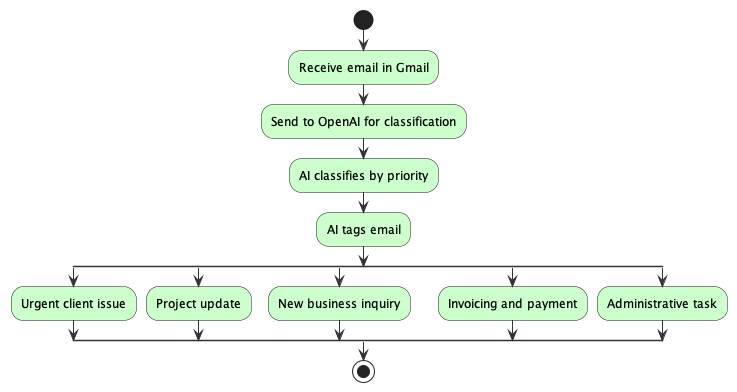
\includegraphics[width=0.8\textwidth]{./figures/01-n8n-flow}
%    \caption{Email Classification and Tagging Automation Flow}
%    \label{fig:email_automation}
%\end{figure}
\begin{tikzpicture}[node distance=1cm, auto]
        % Define styles
    \tikzstyle{startstop} = [rectangle, rounded corners, minimum width=3cm, minimum height=1cm, text centered, draw=black, fill=red!30]
    \tikzstyle{process} = [rectangle, minimum width=3cm, minimum height=1cm, text centered, text width=3cm, draw=black, fill=green!30]
    \tikzstyle{decision} = [diamond, minimum width=3cm, minimum height=1cm, text centered, draw=black, fill=yellow!30]
    \tikzstyle{arrow} = [thick,->,>=stealth]

    % Place nodes
    \node (start) [startstop] {Start};
    \node (receive) [process, below=of start] {Receive email in Gmail};
    \node (send) [process, below=of receive] {Send to OpenAI for classification};
    \node (classify) [process, below=of send] {AI classifies by priority};
    \node (tag) [process, below=of classify] {AI tags email};
    \node (decision) [decision, below=2cm of tag] {};

    \node (project) [process, below left=4cm and 4cm of decision] {Project update};
    \node (inquiry) [process, below left=2cm and 2cm of decision] {New business inquiry};
    \node (admin) [process, below=3cm of decision] {Administrative task};
    \node (invoice) [process, below right=2cm and 2cm of decision] {Invoicing and payment};
    \node (urgent) [process, below right=4cm and 4cm of decision] {Urgent client issue};

    \node (stop) [startstop, below=3cm of admin] {Stop};

    % Draw edges
    \draw [arrow] (start) -- (receive);
    \draw [arrow] (receive) -- (send);
    \draw [arrow] (send) -- (classify);
    \draw [arrow] (classify) -- (tag);
    \draw [arrow] (tag) -- (decision);
    \draw [arrow] (decision) -- (project);
    \draw [arrow] (decision) -- (inquiry);
    \draw [arrow] (decision) -- (admin);
    \draw [arrow] (decision) -- (invoice);
    \draw [arrow] (decision) -- (urgent);
    \draw [arrow] (project) |- (stop);
    \draw [arrow] (inquiry) |- (stop);
    \draw [arrow] (admin) -- (stop);
    \draw [arrow] (invoice) |- (stop);
    \draw [arrow] (urgent) |- (stop);
\end{tikzpicture}

In the following chapters, we'll dive deep into implementing this workflow and many others, step by step.

\section{Join Our Community}

As you embark on this journey, remember that you're not alone. Join our vibrant community of IT consultants and automation enthusiasts on Discord:

\begin{tcolorbox}[colback=secondarylight,colframe=secondarydark,title=Business Automators Community]
    \begin{center}
    \large\url{https://discord.gg/P6txNctp}
    \end{center}

    In our community, you can:
    \begin{itemize}
        \item Get help troubleshooting your automations
        \item Share your own automation success stories
        \item Network with other forward-thinking IT consultants
        \item Get direct access to the author for personalized advice
    \end{itemize}
\end{tcolorbox}

\begin{importantbox}
Remember, automation is a journey, not a destination. Start with the email classification workflow we'll build in the next chapter, then explore how you can automate other aspects of your consulting practice.
\end{importantbox}

Ready to stop drowning in busywork and start leading the pack? Let's dive in!

